% The Clever Algorithms Project: http://www.CleverAlgorithms.com
% (c) Copyright 2013 Jason Brownlee. Some Rights Reserved. 
% This work is licensed under a Creative Commons Attribution-Noncommercial-Share Alike 2.5 Australia License.


% Name
% The algorithm name defines the canonical name used to refer to the technique, in addition to common aliases, abbreviations, and acronyms. The name is used in terms of the heading and sub-headings of an algorithm description.
\section{Ridge Regression} 
\label{sec:ridge}
\index{Ridge Regression}
\index{Tikhonov Regularization}
\index{Tikhonov-Miller Method}
\index{Phillips-Twomey Method}
\index{Constrained Linear Inversion}
\index{Linear Regularization}
\index{Penalized $L_2$ Regression}
\index{$L_2$-norm Penalty}

% other names
% What is the canonical name and common aliases for a technique?
% What are the common abbreviations and acronyms for a technique?
\emph{Ridge Regression, Tikhonov Regularization, Tikhonov-Miller Method, Phillips-Twomey Method, Constrained Linear Inversion, Linear Regularization, Penalized $L_2$ Regression}

% Taxonomy: Lineage and locality
% The algorithm taxonomy defines where a techniques fits into the field, both the specific subfields of Computational Intelligence and Biologically Inspired Computation as well as the broader field of Artificial Intelligence. The taxonomy also provides a context for determining the relation- ships between algorithms. The taxonomy may be described in terms of a series of relationship statements or pictorially as a venn diagram or a graph with hierarchical structure.
\subsection{Taxonomy}
% To what fields of study does a technique belong?
Ridge Regression is a Regularization method for Multiple Linear Regression models.
% What are the closely related approaches to a technique?
Ridge Regression is related to other Regularized Regression models such as the LASSO and Elastic Net.
The general method of penalizing a model based on the sum of squared parameters is related to Weight Decay in the training of Artificial Neural Networks.

% Strategy: Problem solving plan
% The strategy is an abstract description of the computational model. The strategy describes the information processing actions a technique shall take in order to achieve an objective. The strategy provides a logical separation between a computational realization (procedure) and a analogous system (metaphor). A given problem solving strategy may be realized as one of a number specific algorithms or problem solving systems. The strategy description is textual using information processing and algorithmic terminology.
\subsection{Strategy}
% What is the information processing objective of a technique?
The information processing objective of Ridge Regression is to reduce or shrink the magnitude of the coefficients in a regression model.
% What is a techniques plan of action?
This is achieved by penalizing models based on the sum of the squared coefficients called an $L_2$ penalty or the $L_2$ norm. This term is added to the regression equation during the preparation of the model and is weighted by a complexity parameter ($\lambda$) that controls the amount of shrinkage of the coefficients. 
The effect is that coefficients of a regression model are shrunk towards zero during the training of the model. The intercept is not penalized.

% Heuristics: Usage guidelines
% The heuristics element describe the commonsense, best practice, and demonstrated rules for applying and configuring a parameterized algorithm. The heuristics relate to the technical details of the techniques procedure and data structures for general classes of application (neither specific implementations not specific problem instances). The heuristics are described textually, such as a series of guidelines in a bullet-point structure.
\subsection{Heuristics}
% What are the suggested configurations for a technique?
% What are the guidelines for the application of a technique to a problem instance?

\begin{itemize}
	\item It commonly results in a model with a better bias-variance trade-off than Ordinary Least Squares.
	\item The ridge constant $\lambda$ is typically selected in the range $[0,1]$, where $\lambda=0$ corresponds to an Ordinary Least Squares regression.
	\item Unlike other selection methods, Ridge Regression does not drop coefficients, all model parameters are maintained at the end of the process providing shrinkage but not selection of parameters.
	\item Inputs are commonly standardized before training the model as models are not equivalent under scaling.
	\item Cross-validation is commonly used to assess the model and model selection or stopping criteria.
	\item It is suited for problems where there are more predictors $p$ than there are observations $n$, $p>n$ problems.
\end{itemize}

% sample script in R
\subsection{Code Listing}
% listing
Listing~\ref{mass_ridge_regression} provides a code listing of the Ridge Regression method in R.
% algorithm and package
The example uses the \texttt{lm.ridge()} function in the \texttt{MASS} core package which is responsible for fitting linear models using Ridge Regression. The example trials a sequence of lambda values then uses the model with the best lambda value for prediction. Figure~\ref{plot:ridge_regression_result} provides a plot of the final coefficient values of each model for the given lambda values. For more information on this library type: \texttt{library(help="MASS")}, and for more information on the function type: \texttt{?lm.ridge}.

% problem
The test problem is a four-dimensional dataset of 100 samples, where \texttt{x3} and \texttt{y} are dependent on \texttt{x1} and \texttt{x1} and \texttt{x2} are independent variables. The problem is ill defined as \texttt{y} given \texttt{x1, x2, x3}. The model is expected to reduce the contribution of \texttt{x2} and \texttt{x3} toward zero leaving \texttt{y} given \texttt{x1}.

\lstinputlisting[firstline=7,language=r,caption={Example of Ridge Regression in R using the \texttt{lm.ridge()} function in the \texttt{MASS} package.}, label=mass_ridge_regression]{../src/algorithms/regularization/mass_ridge_regression.R}

\begin{figure}[htp]
\centering
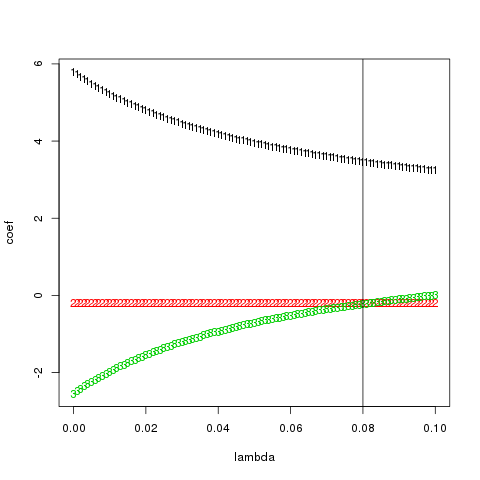
\includegraphics[scale=0.70]{a_regularization/ridge_regression_result.png}
\caption{Plot of the final coefficient values of each model for the given lambda values. The numbers reflect the \texttt{x} variables 1, 2 and 3. The line shows a selected lambda value.}
\label{plot:ridge_regression_result}
\end{figure}

% other packages ?
Other packages that provide an implementation of Ridge Regression include \texttt{parcor}.
% penalized package

% References: Deeper understanding
% The references element description includes a listing of both primary sources of information about the technique as well as useful introductory sources for novices to gain a deeper understanding of the theory and application of the technique. The description consists of hand-selected reference material including books, peer reviewed conference papers, journal articles, and potentially websites. A bullet-pointed structure is suggested.
\subsection{References}
% What are the primary sources for a technique?
% What are the suggested reference sources for learning more about a technique?

% primary sources
\subsubsection{Primary Sources}
% seminal
The method was originally described by Tikhonov \cite{Tikhonov1943, Tikhonov1963} (Russian), who later published a full account of the method as a book \cite{Tikhonov1977}.
% others
Phillips independently described the method \cite{Phillips1962}. Hoerl was first to use the term `Ridge Regression' which was adopted in the field of Statistics for $p>n$ problems \cite{Hoerl1962, Hoerl1970, Hoerl1970a}.

% more info
\subsubsection{More Information}
Hastie et~al.\ provide a gentle introduction to the method from the perspective of linear regression (\cite{Hastie2009}, page 61).
% applied
Press et~al.\ provide an introduction to Ridge Regression with examples in the C programming language \cite{Press2007} (Chapter 19).
Faraway provides an introduction to Ridge Regression with examples in R \cite{Faraway2002}.

% END
